\chapter{Introduction to the Formalization of Fux's Theory}\label{ch:Formalization}
The formalization of Fux is done in several steps:
\begin{enumerate}[wide]
    \item \textbf{Spot the right rules in the \textit{Gradus Ad Parnassum}.} Fux tended to explain certain rules of music so that they were easy to understand and use for the musicians of the time. This implies that sometimes several rules can be reduced to one. On the other hand, some of the rules of music are not written as such in the book because they are implicit. For example, it goes without saying that counterpoint belongs to a certain key and scale, but this is never explicitly written in the book. In order not to create misunderstanding, it was decided to write them explicitly and separately in the next sections.
    \item \textbf{Formalize the rules in natural language in a way that is easy to express as constraints.} Indeed, the \textit{Gradus Ad Parnassum} is a work dedicated to a 17th century audience. It is necessary to read it with a critical eye and to translate it into modern language. That is, to reduce several rules into one, or at times, some rules are expressed in inclusive terms, whereas it is easier for a mathematician or computer scientist to write them in an equivalent way with exclusive terms or vice versa. Examples will be given in section \ref{subsec:1SPEnglish}.
    \item \textbf{On the one hand, write the rules in discrete mathematics.} This is a crucial step in order to be able to use these rules precisely in other contexts and with other programming languages. This will also allow us to check whether solutions exist mathematically. Indeed, some rules may be contradictory and, consequently, no solution would be possible. It is important to keep in mind that some rules are written in a way that can be easily written with the Gecode tool.
    \item \textbf{On the other hand, write the rules in constraint programming language.} The final goal of this thesis is to have constraints fixed according to Fux's rules and to find the best possible solutions with Gecode.
\end{enumerate}

\section{Array Logic and Notation}\label{sec:arrays}
It is particularly important to understand how arrays are constructed. The rest of the paper relies entirely on the nuances and particularities of this logic and notation. This section is intended for mathematicians and computer scientists. 

\subsection{Logic of the arrays}
The majority of the variables are arrays representing "in order" the different constrained values linked to the solution. The solution to the problem is an array of MIDI notes lists representing counterpoint. Before starting, two constants\footnote{Careful, these are constants from the point of view of the Gecode solver. They are variables defined once with the input but which are never set as constraint variables in the CSP.} must be defined\footnote{These constants are defined more precisely in subsection \ref{sec:constants}.}:

\begin{itemize}
    \item $m$ as the number of measures of the \cf and the counterpoint;
    \item $s_{m}$ as the maximum number of notes possible in the counterpoint, i.e. the size of the main arrays used to store Gecode variables. $s_{m} = m + 3\times (m-1)$ and by extension, $s_{m-1} = (m-1) + 3\times (m-2)$.
\end{itemize}

Intuitively one would separate an array into $m$ lists of each measure with the different notes of a measure inside. Here the reverse applies. With a C-like representation, the access to a variable will be done as $[beat][measure]$ instead of $[measure][beat]$. This is more convenient for applying constraints in Lisp with GiL. Indeed, since the number of beats used by species varies, it is then easier to separate the arrays by lists of beats in order to be able to initialize only those which are treated in the problem. Since these arrays are initialized not with simple integers but with \texttt{IntVar} objects from Gecode, these constraint variables would definitely be initialized in the constraint space, which would not be ideal.\\

All the arrays related directly to the counterpoint are stored in arrays of size $s_{m}$ (or $s_{m-1}$ for the melody arrays as will be explained later). These arrays are composed of four lists, each representing the corresponding beat all along the measures of the song. The first is of size $m$ while the other three are of size $m-1$ since they do not have a note in the last measure of the counterpoint which is only composed of a single whole note. E.g. \texttt{notes[0][9]}\footnote{This array exists only as an example. Here the notation corresponds neither to Lisp notation nor to mathematical notation.} would represent the note in the first beat of the tenth measure.

If the chosen species of counterpoint uses only \textbf{whole notes}, i.e. the first one, each note in first beat of each measure lasts \textbf{four beats}. Consequently, the lists of notes in the second, third and fourth beats are not used because these notes would already be represented by the one in first beat. The same logic applies to the other species: the second and fourth species only use the \textbf{first} and \textbf{third} "beat lists" because a note lasts \textbf{two beats}. While the third and fifth species are the only ones to use the \textbf{four available} beat lists because a note (can) last(s) \textbf{one beat}. See figure \ref{fig:thefourspecies} (the corresponding midi value is annotated below each note) and table \ref{tab:thefourspecies} for clarity.
\begin{figure}[h]
    \centering
    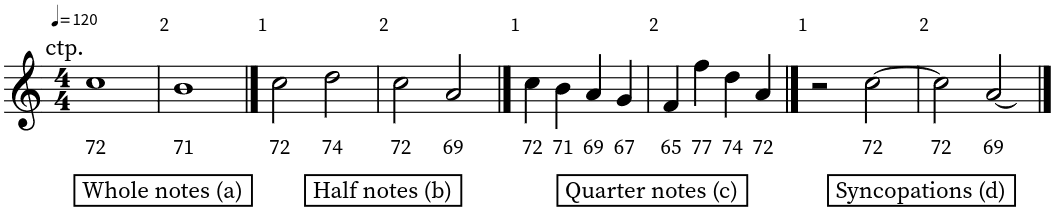
\includegraphics[width=\textwidth]{Images/the_four_species.png}
    \caption{The 3 types of notes (N.B.: b $\equiv$ d) over 8 beats for the \nth{4} first species.}
    \label{fig:thefourspecies}
\end{figure}

\begin{table}[h]
    \centering
    \resizebox{\columnwidth}{!}{%
    \begin{tabular}{|c||c|c|c|c||c|c|c|c|}
        \hline
        beat, measure & \nth{1}, \nth{1} & \nth{2}, \nth{1} & \nth{3}, \nth{1} & \nth{4}, \nth{1} & \nth{1}, \nth{2} & \nth{2}, \nth{2} & \nth{3}, \nth{2} & \nth{4}, \nth{2} \\
        \hline
        \hline
        \hline
        Whole notes & 72 & $\emptyset$ & $\emptyset$ & $\emptyset$ & 71 & $\emptyset$ & $\emptyset$ & $\emptyset$ \\
        \hline
        Half notes & 72 & $\emptyset$ & 74 & $\emptyset$ & 72 & $\emptyset$ & 69 & $\emptyset$\\
        \hline
        Quarter notes & 72 & 71 & 69 & 67 & 65 & 77 & 74 & 72\\
        \hline
        Syncopations & $\emptyset$ & $\emptyset$ & 72 & $\emptyset$ & 72 & $\emptyset$ & 69 & $\emptyset$\\
        \hline
    \end{tabular}
    }
    \caption{Relative MIDI values of figure \ref{fig:thefourspecies}.}
    \label{tab:thefourspecies}
\end{table}

Syncopations have been added to illustrate that they work in the same way as half notes. The fifth species repeats the first four ones so it is not shown here. It will be explained in detail in chapter \ref{ch:5SP}.

\subsection{Notations of the arrays} Several notations exist to describe the elements of an array. The one chosen here is close to the computer notation with the indexing starting at zero.
\begin{multicols}{3}
    \begin{itemize}
        \item $A[i, j]$ for element $j$ of list $i$ of array $A$;
        \item $L[i]$ for element $i$ of list $L$;
        \item $A[i]$ for list $i$ of array $A$.
    \end{itemize}
\end{multicols}

Note that another way is also used to represent all the positions of a table. Indeed, as it is shown in the previous subsection, an array representing all measures per beat can be merged as a long list representing all beats one after the other. Therefore, to clarify the notation, $\forp$ will be used to represent all non-empty positions of an array. For example, for the half notes in the previous table \ref{tab:thefourspecies}: $\rho \in \{[0, 0], [2, 0], [0, 1], [2, 1], \dots\}$. Moreover for notational purposes, $\rho + 1$ will denote the position of the next note such that if $A[\rho] = A[0, 0]$ then $A[\rho + 1] = A[2, 0]$. To explain it properly, the set $\B$ and the constants $b$ and $d$ must be introduced.

\paragraph{$\B$} Set of beats in a measure used by the solver depending on the chosen species. $\B$ can be seen as the location or index of the notes written over a measure on a score.

\begin{equation}
    \begin{gathered}
        \B = \begin{cases}
            \{0\} & \text{if species = 1}\\
            \{0, 2\} & \text{if species = \{2, 4\}}\\
            \{0, 1, 2, 3\} & \text{if species = \{3, 5\}}
            % \{0, 2\} & \text{if species = 4}\\
            % \{0, 1, 2, 3\} & \text{if species = 5}
        \end{cases}
    \end{gathered}
\end{equation}
This refers back to the previous table \ref{tab:thefourspecies}.

\paragraph{b} Number of beat(s) in a measure used by the solver depending on the chosen species. $b$ can be seen as the number of notes written over a measure on a score. $b$ is related to $\B$ since $b = |\B|$.

\begin{equation}
    \begin{gathered}
        b = \begin{cases}
            1 & \text{if species = 1}\\
            2 & \text{if species = \{2, 4\}}\\
            4 & \text{if species = \{3, 5\}}
        \end{cases}
    \end{gathered}
\end{equation}

\paragraph{d} Duration of a note in beat(s) depending on the chosen species. $d$ can be seen as the space between the notes of a measure on a score. $d$ is inversely proportional to $b$.

\begin{equation}
    \begin{gathered}
        d = 4/b\\
        \therefore d = \begin{cases}
            4 & \text{if species = 1}\\
            2 & \text{if species = \{2, 4\}}\\
            1 & \text{if species = \{3, 5\}}
        \end{cases}
    \end{gathered}
\end{equation}

\paragraph{positions(upto)} Function that returns the set of non-empty positions or indexes ordered depending on the species in such a way that all the positions would follow one another to represent all the beats of that species on a score in a single list.

\begin{equation}
    \begin{gathered}
        % \forall i \in \B, \forall j \in upto\\
        positions(upto) = \bigcup _{\forall i \in \B, \forall j \in [0, upto)} [i, j]\\
        \text{s.t. } \forall x \in [1, 3], \forall y \in [1, upto)\\
        [i, j] <_{s} [i + x, j] <_{s} [i, j + y]\\
        \text{where } <_{s} \text{ means the sorting order}\\
    \end{gathered}
\end{equation}
By extension, $\rho + z >_{s} \rho$ such that:

\begin{equation}
    \begin{gathered}
        \forall z \in \mathbb{N}^+, \forall \rho = [i, j] \in positions(upto)\\
        \rho + z = [i + zd, j + nextm(i+zd)]\\
        \text{where } nextm() \text{ is a function that returns the correct number of measure(s) to add.}
    \end{gathered}
\end{equation}
\section{Definitions of the Constants, Costs, Variables and Functions}
This section is more intended for mathematicians and computer scientists too. Those who don't wish to read the mathematical parts should still broadly understand the variables of harmonic intervals, melodic intervals and motions (\textbf{H}, \textbf{M} and \textbf{P} in section \ref{sec:variables}). Subsections \ref{sec:constants} and \ref{sec:variables} describes the various names used in the mathematical parts and in the Lisp code of the solver (immediately to their right, e.g. \textbf{n} \space \texttt{*total-cp-len}). These subsections explain also how those constants and variables work. Unless otherwise stated, all domains of constants and variables belong to the domain of integers $\mathbb{N}$.

% CONSTANTS
\subsection{Constants}\label{sec:constants}
Constants are only constant with respect to the Gecode solver, so they are deduced before a solution is sought by the latter.

\paragraph{Cons $_{(all,\ p,\ imp)}$} \texttt{ALL\_CONS}, \texttt{P\_CONS}, \texttt{IMP\_CONS}

Set representing all consonances, perfect consonances and imperfect consonances respectively. By default, the notation $Cons \equiv Cons_{all}$.

\begin{equation}
    \begin{gathered}
        Cons_{p} := \{0, 7\}\\
        Cons_{imp} := \{3, 4, 8, 9\}\\
        Cons_{all} := Cons_{p} \cup Cons_{imp} \equiv \{0, 3, 4, 7, 8, 9\}
    \end{gathered}
\end{equation}

\paragraph{species} \texttt{species}

Chosen species of counterpoint. $species \in \{1, 2, 3, 4, 5\}$.

\paragraph{m} \texttt{*cf-len}

Number of measures which is equivalent to the number of notes in the \cfdot $m \in [3, 17]$. $3$ because the solver needs al least 3 measures to work properly. $17$ is arbitrary and comes from $4\times 4 + 1$, i.e. a commun number of measure $\times$ a number not too large for the computation $+$ one final measure.

\paragraph{n} \texttt{*total-cp-len}

Number of notes in the counterpoint depending on the chosen species. $n \in [1, b(m-1)+1]$ because the last measure has necessarily a whole note.

\paragraph{s$_{m}$}

Maximum number of notes contained in the counterpoint, all species combined, i.e. if the counterpoint contained only quarter notes, with the exception of the last note being a whole note.

\begin{equation}
    s_{m} = m + 3\times (m-1) \text{ and }s_{m-1} = (m-1) + 3\times (m-2)
\end{equation}

Used as the size for an array containing one list of size $m$ (or $m-1$) the notes in thesis and three lists of size $m-1$ (or $m-2$) the other beats. The difference with $n$ is that $s$ does not depend on $b$.

\paragraph{Cf} \texttt{*cf}

List of size $m$ representing the MIDI notes of the \cfdot

\begin{equation}
    \begin{gathered}
        \forall j \in [0, m)\\
        Cf[j] \in [0, 127]
    \end{gathered}
\end{equation}

\paragraph{M$_{cf}$} \texttt{*cf-brut-m-intervals}

List of size $m-1$ representing the melodic intervals between the consecutive notes of the \cfdot

\begin{equation}
    \begin{gathered}
        \forj\\
        M_{cf}[j]=Cf[j+1]-Cf[j]\\
        \text{where } M_{cf} \in [-127, 127]
    \end{gathered}
\end{equation}
% N.B.: any melodic interval should ideally be in the range $[-12, 12]$.

\paragraph{lb} \texttt{RANGE\_LB}

Lower bound of the range of the notes of the counterpoint. $lb \in [0, ub)$.

\paragraph{ub} \texttt{RANGE\_UB}

Upper bound of the range of the notes of the counterpoint. $ub \in (lb, 127]$.

\paragraph{$\R$} \texttt{*cp-range}

Range of the notes of the counterpoint. $\R := [lb, ub]$.

\paragraph{borrow} \df{major}\footnote{\df{value} means the default value in the tool.}

Determines the "borrowing scale", i.e. the additional notes that the counterpoint can have in relation to the tonic of the piece. More details will be given on what are the borrowed notes in section \ref{sec:generalenglish}.

\begin{equation}
    \begin{gathered}
        borrow \in \{none, major, minor\}
    \end{gathered}
\end{equation}

\paragraph{$\N_{(all,\ key,\ brw)}^{(\R)}$} \texttt{*extended-cp-domain}, \texttt{*scale}, \texttt{*borrowed-scale}.

Set of values available for the notes of the counterpoint. $\N_{key}$ represents the notes of the key provided by the user's score. $\N_{brw}$ represents the additional borrowed notes that the counterpoint can have in relation to the tonic of the piece. $\N_{all}$ represents the union of the two previous sets. If $borrow = none$ then $\N_{brw} = \emptyset$ and $\N_{all} = \N_{key}$. $\N_{(all,\ key,\ brw)}^{\R}$ represents the set of notes bounded to the range, i.e. the intersection of $\N_{(all,\ key,\ brw)}$ and $\R$. By default, $\N$ refers to $\N_{all}$ not bounded to the range.

\begin{equation}
    \begin{gathered}
        \N_{key} := buildScale(key, scale)\\
        \N_{brw} := \begin{cases}
            \emptyset & \text{if } borrow = none\\
            buildScale(Cf[0]\ mod\ 12, "borrowed") & \text{if } borrow = major\\
            buildScale([Cf[0]+3]\ mod\ 12, "borrowed") & \text{if } borrow = minor
        \end{cases}\\
        \N_{all} := \N_{key} \cup \N_{brw}\\
        \N_{(all,\ key,\ brw)}^{\R} := \N_{(all,\ key,\ brw)} \cap \R\\
    \end{gathered}
\end{equation}

Where $buildScale(key, scale)$ (see function \ref{eq:buildScale}) is a function that returns the set of notes in the $key$ based on the $scale$ used. Also more details on the borrowed notes will be given in section \ref{sec:generalenglish}.

\subsection{Costs}
The costs are constants chosen by the user that have default values supposed to represent Fux's preferences.

\paragraph{pref and cost} \texttt{*params*}

A preference can have 7 levels of intensity ranging from "no cost" to "forbidden". For any cost $cost$ and any preference $pref$, it can be defined that:

\begin{equation}
    \begin{gathered}
        cost = \begin{cases}
            0 & \text{if } pref = \text{no cost}\\
            1 & \text{if } pref = \text{low cost}\\
            2 & \text{if } pref = \text{medium cost}\\
            4 & \text{if } pref = \text{high cost}\\
            8 & \text{if } pref = \text{last resort}\\
            2m & \text{if } pref = \text{cost prop. to length}\\
            64m & \text{if } pref = \text{forbidden}
        \end{cases}
    \end{gathered}
\end{equation}

$64m$ is a ridiculously huge value that will never be reached by all the other costs combined even if they were all high.

\paragraph{Cond$_{costs}$ and cost$_{Cond}$} All costs work the same way: a list of boolean variables, called $Cond$ for the explanation, determines whether it is true that a certain cost should be established for this specific condition in certain locations. The list of assigned costs for this condition is noted $Cond_{costs}$. The elements of $Cond_{costs}$ are thus equivalent to any cost $cost$ depending on the preference $pref$ chosen for the condition $Cond$. The different costs for the different types of conditions each have their own identifier noted $cost_{Cond}$. It is this value that changes depending on the user's preference. To sum up:

% \begin{equation}
%     \begin{gathered}
%         \forall c \in Cond_{costs}, \forall cond \in Cond\\
%         c = \begin{cases}
%             cost_{Cond} & \text{if } cond \text{ is true}\\
%             0 & \text{otherwise}
%         \end{cases}\\
%         \text{where } cost_{Cond} \in dom(cost)
%     \end{gathered}
% \end{equation}

\begin{equation}
    \begin{gathered}
        \forall \rho \in Positions(Cond)\\
        Cond_{costs}[\rho] = \begin{cases}
            cost_{Cond} & \text{if } Cond[\rho] \text{ is true}\\
            0 & \text{otherwise}
        \end{cases}\\
        \text{where } Positions(Cond) \text{ is the set of positions where the condition } Cond \text{ applies}\\
        \text{ and where } cost_{Cond} \in dom(cost)
    \end{gathered}
\end{equation}

\paragraph{$\C$ and $\tau$} \texttt{*cost-factors}, \texttt{*total-cost}.

The heuristic of the solver leads to find a solution while minimizing the total cost. The latter is represented by $\tau$ while $\C$ is a set of integers representing all the sums of the different lists of costs. $\tau$ is thus the sum of all the elements of $\C$. If $Costs$ is the set of all the different $Cond_{costs}$ lists then:

\begin{equation}
    \begin{gathered}
        \C = \bigcup _{\forall \chi \in Costs} \ \sum _{\forall c \in \chi} c\\
        \tau := \sum _{\forall \sigma \in \C} \sigma\\
        \min \tau
    \end{gathered}
\end{equation}

By definition, for any forbidden $pref$ to be indeed \emph{forbidden}, the following constraint must be added:

\begin{equation}
    \begin{gathered}
        \sum _{\forall \sigma \in \C} \sigma < 64m
    \end{gathered}
\end{equation}

% VARIABLES
\subsection{Variables}\label{sec:variables}
Variables are fully deduced by the Gecode solver and their values can be evaluated only after a solution has been found.

Many variables have a general definition so that they can be used in all equations, this does not mean that all possible combinations have been defined in the Lisp code but only those that are actually used. For example, there is no need to have access to all possible melodic intervals in the solver, however the mathematical notation would allow it.

If some letters are not defined, it means that they have already been defined in the constants or in the previous variables.
\paragraph{Cp} \texttt{*cp} %%% COUNTERTPOINT %%%

Array of size $s_{m}$ representing the MIDI notes of the counterpoint. This array is thus composed of four lists, each representing a beat on all the measures of the song. As explained above, this is how all the other arrays related to the countrepoint (i.e. the $Cp$ array) are constructed.

For example, for a whole notes counterpoint: the relevant $Cp$ would be only the list $Cp[0]$. For a half notes counterpoint: it would be the merge of $Cp[0]$ and $Cp[2]$. For a quarter notes counterpoint: it would be the merge of $Cp[0]$, $Cp[1]$, $Cp[2]$ and $Cp[3]$.

\begin{equation}
    \forall i \in \B, \forall j \in [0, m): Cp[i, j]\in \N^{\R}
\end{equation}

Figure \ref{fig:solverdiagram} shows a popularization of the tool's logic vis-à-vis these arrays of variables.

\begin{figure}
    \centering
    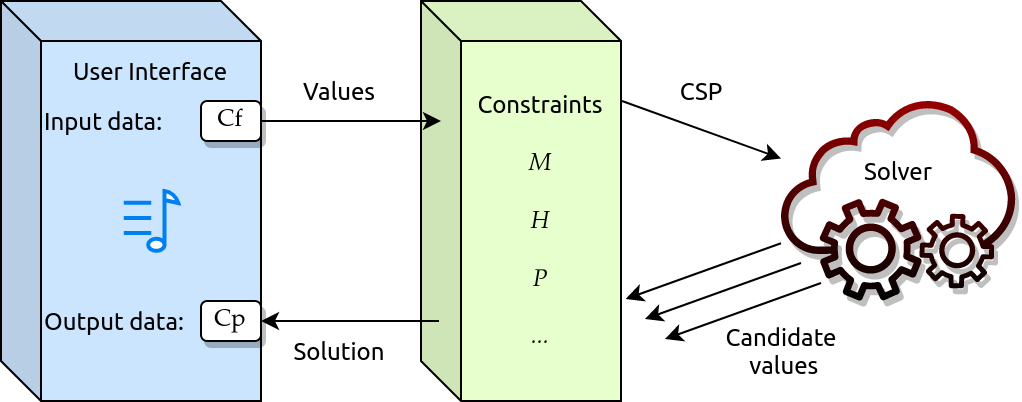
\includegraphics[height=1.7in]{Images/solver_diagram.png}
    \caption{Popularization of the tool's logic vis-à-vis the arrays of variables.}
    \label{fig:solverdiagram}
\end{figure}

\paragraph{H$_{(abs)}$} \texttt{*h-intervals, *h-intervals-abs.} %%% HARMONIC INTERVALS %%%

Array of size $s_{m}$ representing each harmonic interval between the counterpoint and the \cfdot There are four lists of harmonic intervals, each representing a beat along the whole counterpoint. The harmonic intervals are calculated so that they represent the absolute difference between the pitch of the counterpoint and the pitch of the \cfdot Since the values are absolute, it does not matter if the \cf is lower or upper, the intervals will always be calculated according to the lowest note. Any harmonic interval is calculated according to the notes played at the same time in the \cf and the counterpoint. Therefore, up to four notes in the counterpoint can be calculated with respect to the same note in the \cfdot

Two versions of that array-variable exist: the main one $H$ which is modulo 12 and $H_{abs}$ which is not. It is always true that $H = H_{abs}\ mod\ 12$. Unless mentioned, when talking about "harmonic intervals" or "harmonies", it refers to the variables of the array $H$.

\begin{equation}
    \begin{gathered}
        \forall i \in \B, \forall j \in [0, m)\\
        H_{abs}[i, j] = \left|Cp[i, j] - Cf[j]\right|\\
        H[i, j] = H_{abs}[i, j]\ mod\ 12\\
        \text{where } H_{abs}[i, j] \in [0, 127], H[i, j] \in [0, 11]
    \end{gathered}
\end{equation}

$12$ representing the number of semitones in an octave. This allows the interval between a note and any note higher at different octaves to always be the same. This implies that $H \in$ table \ref{tab:intervalsvalues} values. For example, for the gap between $C_4$ (60) and $G_4$ (67) and the gap between $C_4$ (60) and $G_5$ (79), the $H_{abs}$ values will be 7 and 19 while the $H$ values will be 7 and 7.

\begin{figure}[h]
    \centering
    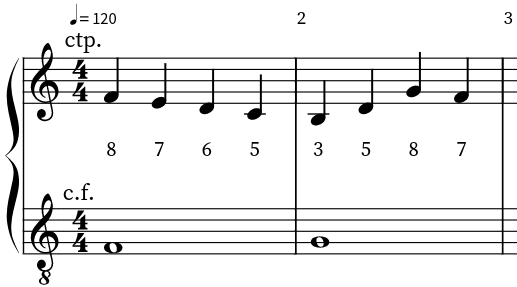
\includegraphics[width=2.5in]{Images/harmonic_intervals_variables.png}
    \caption{Traditionally written harmonies between the ctp. and the \cfdot}
    \label{fig:harmonicintervals}
\end{figure}

Beware that the numbers noted on figure \ref{fig:harmonicintervals} are those used on scores. They refer to the names of the intervals and not to the relative MIDI values. By contrast, table \ref{tab:hjarrayvar} below shows the MIDI values of the intervals for this figure.

\begin{table}[h]
    \centering
    \begin{tabular}{|c||c|c|c|c|}
    \hline
    measure $j$ & $H_{abs}[0, j]$ & $H_{abs}[1, j]$ & $H_{abs}[2, j]$ & $H_{abs}[3, j]$ \\ \hline
    0 & 12 & 11 & 9 & 7 \\ \hline
    1 & 4 & 7 & 12 & 10 \\ \hline
    \end{tabular}
    \caption{Relative MIDI values of figure \ref{fig:harmonicintervals}.}
    \label{tab:hjarrayvar}
\end{table}

\paragraph{M$^{(x)}_{(brut)}$} %%% MELODIC INTERVALS %%%

\texttt{*m-intervals, *m-intervals-brut, *m2-intervals, \dots}
%  *m2-intervals-brut,\\
% *m-succ-intervals, *m-succ-intervals-brut.}

Arrays of size $s_{m-x}$ representing each melodic interval between a note of the counterpoint at a specific beat and another further note of the counterpoint at another specific beat. The melodic intervals are calculated so that they represent the difference between the two notes involved.

The array is noted $M^x$ where $x$ is the number of $d$\footnote{Duration of a note in beat(s) depending on the chosen species (see $d$ in above section \ref{sec:constants}).} beat(s) that separates the initial note to the further one. $x$ represents the desired number of notes between the current note and the one of interest to calculate the melodic interval. In other words, $M^x[i, j]$ represents the melodic interval between the note at beat $i$ in measure $j$ and the note at beat $[(i+xd)\ mod\ 4]$ in measure $[j+nextm(i+xd)]$. If $x$ is not present then its default is 1. For example, with whole notes (i.e. $d=4$): $M[0, 5]$ represents the melodic interval between the note in the sixth measure ($j=5$) and the note in the seventh measure ($j=6$).

There are two versions of that array-variable: the main one $M^x$ which is absolute and $M^x_{brut}$ which is not. It is always true that $M^x = \left|M^x_{brut}\right|$. Unless mentioned, when talking about "melodic intervals" or "melodies", it refers to the variables of the array $M^1$. See figure \ref{fig:threetypesofnotes} (the corresponding midi value is annotated below each note) and table \ref{tab:mxarrayvar} for clarity.
\begin{equation}
    \begin{gathered}
        \forall x \in \{1, 2\}, \forall i \in \B, \forall j \in [0, m-x)\\
        M^x_{brut}[i, j] = Cp[(i+xd)\ mod\ 4, j+nextm(i+xd)] - Cp[i, j]\\
        M^x[i, j] = \left|M^x_{brut}[i, j]\right|\\
        \text{where } M^x_{brut}[i, j] \in [-12, 12], M^x[i, j] \in [0, 12]
    \end{gathered}
\end{equation}

The intervals are limited to $12$ because the octave leap is the maximum that can be reached.

\begin{figure}[h]
    \centering
    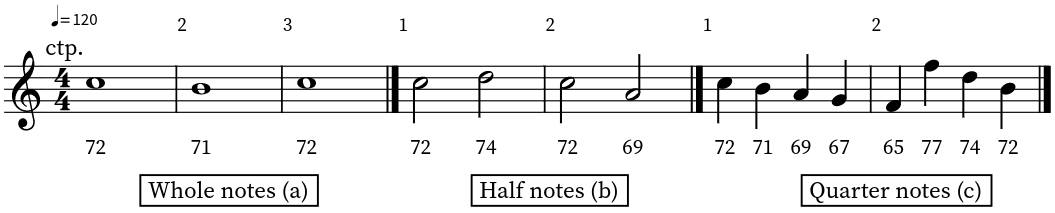
\includegraphics[height=1in]{Images/melodic_intervals_variables.png}
    \caption{The 3 types of notes that can be used in the counterpoint.}
    \label{fig:threetypesofnotes}
\end{figure}

\begin{table}[h]
    \centering
    \begin{tabular}{|c|||c||c||c|}
    \hline
    $M^x_{(brut)}$      & Whole notes (a) & Half notes (b) & Quarter notes (c) \\ \hline \hline
    $M[0, 0]$   & 1 (-1)        & 2 (2)          & 1 (-1)            \\ \hline
    $M[1, 0]$   & $\emptyset$   & $\emptyset$    & 2 (-2)            \\ \hline
    $M[2, 0]$   & $\emptyset$   & 2 (-2)         & 2 (-2)            \\ \hline
    $M[3, 0]$   & $\emptyset$   & $\emptyset$    & 2 (-2)            \\ \hline
    $M[0, 1]$   & 1 (1)         & 3 (-3)         & 12 (12)            \\ \hline
    $M^2[0, 0]$ & (0)           & 0 (0)          & 3 (-3)            \\ \hline
    $M^2[2, 0]$ & $\emptyset$   & 5 (-5)         & 4 (-4)            \\ \hline
    \end{tabular}
    \caption{Some relative MIDI values of figure \ref{fig:threetypesofnotes} with $x=\{1, 2\}$.}
    \label{tab:mxarrayvar}
\end{table}

In the solver, melodic intervals used are stored in several lists by beat pair, e.g. one list for all the intervals between the first and second beats of all measures. The constraints to represent these calculations are done separately from one table to another with the same function. From example, all the melodic intervals between the fourth beat note and the next first beat note in the thrid species are computed like in equation \ref{eq:melo30example}:

\begin{equation}
    \begin{gathered}
        \forj\\
        M_{brut}[3, j] = Cp[0, j+1] - Cp[3, j]\\
        M[3, j] = \left|M_{brut}[3, j]\right|\\
    \end{gathered}
    \label{eq:melo30example}
\end{equation}

\paragraph{P} \texttt{*motions} %%% MOTIONS %%%

Array of size $4\times (m-1)$ representing each motion between two consecutive measures. The letter $P$ is for \textit{passage} since $M$ is already taken.
% The motions are calculated in such a way that they directly represent the cost of themselves. By default, contrary motions are the most appreciated and have no cost. Oblique motions are not restricted and have a cost of 1. Direct motions are less appreciated and have a cost of 2.
Contrary, oblique and direct motions are represented by 0, 1 and 2 respectively.

\begin{equation}
    \begin{gathered}
        \forall x \in \{1, 2\}, \forall i \in \B, \forj, x := b-i\\
        P[i, j] =
        \begin{cases}
            0 & \text{if } (M^{x}_{brut}[i, j] > 0 > M_{cf}[j]) \lor (M^{x}_{brut}[i, j] < 0 < M_{cf}[j]) \\
            1 & \text{if } M^{x}_{brut}[i, j] = 0 \lor M_{cf}[j] = 0 \\
            2 & \text{if } (M^{x}_{brut}[i, j] > 0 \land M_{cf}[j] > 0) \lor (M^{x}_{brut}[i, j] < 0 \land M_{cf}[j] < 0)
        \end{cases}
        % \text{where } P[i, j] \in \{0, 1, 2\}
    \end{gathered}
\end{equation}

$x:=b-i$ represents the fact that the motion is obtained between the current note and the first note of the next measure. For example, with quarter notes, the gap between the third note and the first note of the next measure is defined as: $b=4$, $i=2$ and $x=4-2=2$. The first note of the next measure is therefore 2 notes away.

The motions require relatively many constraints to be computed. Indeed, a boolean variable is needed for each type of direction of the counterpoint melody (3) as well as that of the \cf (3). This gives 3*3 different possibilities to be divided into 3 categories of motions for each measure. This is not a problem in itself but with GiL, any boolean operation must be computed via a constrained boolean variable. Ideally one should use argument variables provided by Gecode that are intended to be temporary variables. Implementing this in GiL would probably improve performance.

\paragraph{IsCfB} \texttt{*is-cf-bass-arr}

Boolean array of size $s_{m}$ representing if the \cf is below. Each list of this array represents a beat along the whole counterpoint and is calculated by comparing the pitch of the counterpoint with the pitch of the \cf at the same time.

\begin{equation}
    \begin{gathered}
    \forall i \in \B, \forall j \in [0, m)\\
    IsCfB[i, j] =
    \begin{cases}
        \top & \text{if } Cp[i, j] \geq Cf[j] \\
        \bot & \text{otherwise}
    \end{cases}
    \end{gathered}
\end{equation}

By default, if both notes are the same then the \cf is considered as the bass.

\paragraph{IsCons$_{(all,\ p,\ imp)}$} \texttt{*is-cons-arr}

Boolean array of size $s_{m}$ representing if harmonic intervals are consonances, perfect consonantes or imperfect consonances. Each list of this array represents a beat along the whole counterpoint and is calculated by checking that harmonies belong to the corresponding set of consonances. By default, $IsCons \equiv IsCons_{all}$.

\begin{equation}
    \begin{gathered}
    \forall i \in \B, \forall j \in [0, m)\\
    IsCons[i, j]_{(all,\ p,\ imp)} =
    \begin{cases}
        \top & \text{if } H[i, j] \in Cons_{(all,\ p,\ imp)}\\
        \bot & \text{otherwise}
    \end{cases}
    \end{gathered}
\end{equation}

% FUNCTIONS
\subsection{Fonctions}
Functions are a way to improve the readability of some more complex mathematical notations. The majority remain relatively simple.
\paragraph{nextm(x)} Returns the number of measure(s) to add in 4/4 time signature depending on the number of beat $x$.
\begin{equation}
    nextm(x) = \begin{cases}
        1 + nextm(x-4)& \text{if } x \geq 4\\
        0 & \text{otherwise}
    \end{cases}
    \label{eq:nextm}
\end{equation}

\paragraph{buildScale(key, scale)} Returns the set of notes in the $key$ based on the $scale$ used. $key$ is a value between 0 and 11 such that $0 \equiv C$ and $11 \equiv B$.

\begin{equation}
    \begin{gathered}
        \forall x \in [-11, 127], \forall \delta := key+x \in [0, 127]\\
        buildScale(key, scale) = \begin{cases}
            \bigcup _{\delta\ mod\ 12 \in key + \{0, 2, 4, 5, 7, 9, 11\}} \delta & \text{if } scale = \text{major}\\
            \bigcup _{\delta\ mod\ 12 \in key + \{0, 2, 3, 5, 7, 8, 10\}} \delta & \text{if } scale = \text{minor}\\
            \bigcup _{\delta\ mod\ 12 \in key + \{0, 5, 9, 11\}} \delta & \text{if } scale = \text{borrowed}
        \end{cases}\\
        \text{where } key \in [0, 11], scale \in \{"major", "minor", "borrowed"\}
    \end{gathered}
    \label{eq:buildScale}
\end{equation}
N.B.: $buildScale(key, "minor") \equiv buildScale([key+3]\ mod\ 12, "major")$.

\paragraph{Membership function $e \in E$} State that $e$ belongs to $E$. Technically, that's a fact but, \emph{in the context of this paper}, this function can be used as a boolean function to evaluate an implication. It is then considered that this function returns a boolean value that is true if $e$ is in the set $E$.

\begin{equation}
    \begin{gathered}
        E := \{e_0, \dots, e_n\}\\
        e \in E = \begin{cases}
            \top & \text{if } (e = e_0) \lor \dots \lor (e = e_n)\\
            \bot & \text{otherwise}
        \end{cases}
    \end{gathered}
\end{equation}

As a result, when an expression uses only $\in$, it implies that this expression is true, i.e the element must belong to the set: $e \in E \equiv (e \in E \iff \top)$. This refers directly to the way Gecode allows this constraint. It may not follow convention, but it will be simpler and still used with common sense.

In the code, the constraints are often expressed separately for each element. For example, for a constraint $cst$ which is applied if $e \in \{x, y, z\}$, it would state:

\begin{equation*}
    \begin{gathered}
        (e = x) \implies cst;\quad (e = y) \implies cst;\quad (e = z) \implies cst
    \end{gathered}
\end{equation*}
\section{Implicit General Rules of Counterpoint}

\paragraph{}In this section, all the following rules are implicit, sometimes taken from Fux's examples, and sometimes from music theory in general.

\subsection{Formalization in English} \label{sec:generalenglish}
\begin{enumerate}[wide, label=\bfseries G\arabic*]
    \item \textit{Harmonic intervals are always calculated from the lower note.} \label{rule:hfromlower}

    Indeed, any harmonic interval is a calculation of the absolute difference between two notes. This implies that they adapt to where the counterpoint is in relation to the \cfdot.

    \item \textit{The number of measures of the counterpoint must be the same as the number of measures of the \cfdot} \label{rule:sameNbMeasures}

    The goal is to compose complete counterpoints which last the same time as the \cfdot

    \item \textit{The counterpoint must have the same time signature and the same tempo as the \cfdot} \label{rule:sameTimeSignature}

    The notes must be played in sync.

    \item \textit{The counterpoint must be in the same key as the \cfdot}\label{rule:samekey}

    This is a fundamental rule of music in general. Since the music of the Baroque period does not follow the same standards as today's music, this rule is a bit more complicated than it seems. Indeed, it often happens that Fux gives examples with accidentals, i.e. notes that do not belong to the diatonic scale. There are therefore notes "borrowed" from other scales which do not appear as a basis for the key signature.
    \begin{figure}[h]
        \centering
        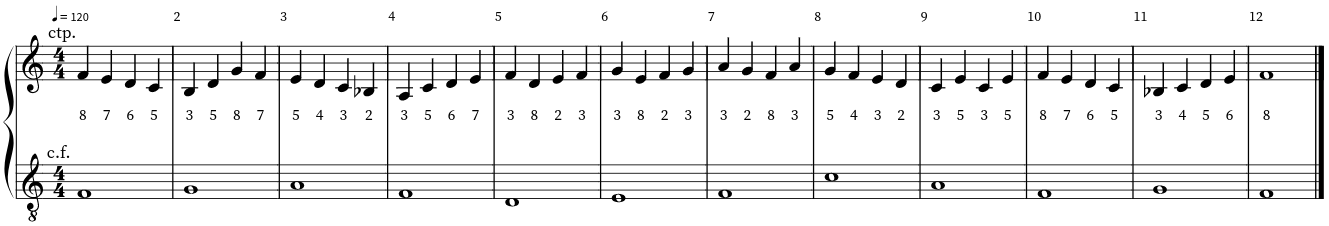
\includegraphics[width=\textwidth]{Images/mode_deter_by_first_note.png}
        \caption{Example of a $C$ major key signature starting on $F$ with $B\flat$'s \parencite[p.54]{GaPEng}.}
        \label{fig:mode_determined}
    \end{figure}

    This makes it somewhat difficult to determine the precise domain of notes available for counterpoint. It is possible to determine the logic behind these borrowed notes. One way of looking at it is as follows: Fux composes with several different modes throughout his work: the $F$ (Lydian) mode, the $D$ (Dorian) mode, and others. In the rules of the first species (see section \ref{subsec:1SPEnglish} at \ref{rule:keytone}), it will be seen that Fux determines the use of a mode according to the first note of the \cf in relation to the key of the musical work. Since the nature of a mode can be either major or minor, some notes can be borrowed from the major or minor diatonic scale of the first note of the \cf respectively.

    In figure \ref{fig:mode_determined}, the key is $C$ major, i.e. [$C, D, E, F, G, A, B$]. These notes can therefore be used in counterpoint, but that is not all. Since the first note is an $F$, this implies that the tonic of this work is $F$, although it uses the major scale of $C$, so it is an example of the use of the $F$ mode, the Lydian mode. The Lydian mode being a major mode, some notes of the diatonic major scale of $F$ can be used sparingly by counterpoint. Looking at several examples given by Fux, the notes borrowed are I ([$F$]\footnote{Notes corresponding to the example are put in square brackets.} necessarily included since it determines the tonic of the work), IV ([$B \flat$] the fourth), VI ([$D$] note of the relative minor) and VII ([$E$] the sensible which is most often used in the penultimate measure). These notes are probably not arbitrary, but for the purposes of this work, it is simply the examples provided by Fux that allow to say that these notes can be used sparingly if necessary.

    If the key notes and the borrowed notes are merged, then the following set of notes is got: [$C, D, E, F, G, A, B \flat, B$]. Since the modes are variations of the diatonic scale, only a few notes are added in the end (one in this case).
    It is more complicated to understand when exactly these borrowed notes are used. Fux explains that these notes can be used to avoid certain intervals at certain times, which otherwise the melody would harshly imply the relationship of \textit{mi} against \textit{fa} \parencite[p.35]{GaPEng}. Again, his approach to music is probably stricter than the current one, especially when his music was intended to be religious songs. That is why this setting is user-definable.

    \item \textit{The range of the counterpoint must be consistent with the instrument used.} \label{rule:instrurange}

    This rule is relatively arbitrary and should be managed by the software user. Fux's treatise is mainly concerned with sung counterpoint, although it is applicable to any instrument. Most of the time, counterpoint is composed either in a higher register or in a lower register and more rarely both simultaneously. For performance reasons, the range in the software is limited to a size of one and a half octaves, i.e. 18 semitones. Which is in itself completely consistent with the style of counterpoint. The user still has the choice of the general pitch of the generated melody.

    \item \textit{Chromatic melodies are forbidden.}\label{rule:chromafb}

    In this work, a melody is considered chromatic when three notes in a row are separated by semitones in the same direction. For example, $C\to C\sharp\to D$ or $C\to B\to B\flat$ are chromatic melodies. As a rule, this should never happen because the diatonic scale does not have those intervals. However, it might be possible to compose chromatic melodies by using borrowed notes in the use of certain modes.
    
    \item \textit{Melodic intervals should be small.}\label{rule:smallmelody}

    The purpose of a melody is to be melodious, but how to define that? This question is several centuries old and still does not have an answer that suits everyone.
    % Some people see melody as a rapid sequence between tension and rest \parencite{Melody}. Others think that the repetition of a motif is essential. Depending on the musical context, it is impossible to define precise rules that work for sure. It is therefore important to see these rules as advices rather than as absolute rules. But how do you represent advice with constraints? One solution is to promote some intervals over others.\\
    In his treatise, Fux argues that one should never neglect the beauty of singing. As a result according to his examples, most melodies consist of stepwise\footnote{Which moves by scale steps (i.e. one tone or one semitone)\parencite{Step}.} motions with occasional leaps. One solution to represent this is to a give higher cost to larger melodic intervals. The appropriate cost function will be discussed in each chapter of species.
    
    % \item \textit{Penultimate notes of the counterpoint tend to rise.} \label{rule:penultrise}

    % While at the end the \cf tends to fall, the counterpoint tends to rise. It makes sense because the last motion must always be contrary (or oblique as will be seen in the next chapter). In Fux's examples, most of them tend to confirm this trend for the last two or even three notes of the counterpoint depending on the species. The examples given in this thesis are therefore strongly influenced by this idea which is omnipresent in the \citetitle{GaPFr}.
\end{enumerate}

\subsection{Formalization into Constraints}

\paragraph{\ref{rule:hfromlower}} \textit{Harmonic intervals are always calculated from the lower note.}

Already handled by making the difference value absolute as seen in section \ref{sec:variables} for the \textbf{H} variable. 

\paragraph{\ref{rule:sameNbMeasures}, \ref{rule:sameTimeSignature}} \textit{Same number of measures and same time signature.}

Only 4/4 time signatures are currently considered. The array $Cp$ is therefore composed of four lists as explained in section \ref{sec:variables} at \textbf{Cp}.

\begin{lstlisting}[caption=Definition of $Cp$ in the first species., label=lst:defcp, basicstyle=\ttfamily\small]
(defvar *cp (list nil nil nil nil))
; ...
;; FIRST SPECIES ;;
; setting the first list of *cp with
;   integer *cf-len as size
;   set *extended-cp-domain as available notes
(setf (first *cp)
    (gil::add-int-var-array-dom *sp* *cf-len *extended-cp-domain))
\end{lstlisting}

\paragraph{\ref{rule:samekey}} \textit{The counterpoint must be in the same key as the \cfdot}

This rule is already handled by the creation of the set $\N$ as shown in section \ref{sec:variables}. The example of the actual rule given above will clarify the explanations. Let $k$ be the value of the key determined by the key signature, i.e. $60$ for $C$; and $t$ the tonic of the piece, i.e. $Cf[0]=65$. Then:

\begin{equation*}
    \begin{gathered}
        \N_{key} = buildScale(k\ mod\ 12, "major") = \{0, 2, 4, 5, 7, 9, 11, 12, \dots, 127\}\\
        \N_{brw} = buildScale(t\ mod\ 12, "borrowed") = \{2, 4, 5, \textbf{10}, 14, \dots, 125\}\\
        \therefore \N_{all}=\{0, 2, 4, 5, 7, 9, \textbf{10}, 11, 12, \dots, 127\}
    \end{gathered}
\end{equation*}

To ensure that borrowed notes are used sparingly, they must be given a cost to use. Let $OffKey$ be the set of notes outside the key and $OffKey_{costs}$ the list of costs associated with each note. The cost for a note will be \textit{<no cost>} or $cost_{OffKey}$ (\dft{high cost}).

\begin{equation}
    \begin{gathered}
        OffKey = [0, 1, 2, \dots, 127] \setminus \N_{key}\\
        % \forall c \in OffKey_{costs}, \forall p \in Cp \\
        % \forall \rho \in \mathcal{P}ositions\\
        \forp\\
        OffKey_{costs}[\rho] = \begin{cases}
            cost_{OffKey} & \text{if } Cp[\rho] \in OffKey \\
            0 & \text{otherwise}
        \end{cases}\\
        \text{moreover } \C = \C \cup \sum _{c \in OffKey_{costs}} c
    \end{gathered}
\end{equation}

This equation is trivial but requires several adjustments in the program. Indeed, there is no boolean constraint in Gecode that assign the value \emph{true} to a variable if an element belongs to a set\footnote{To our knowledge, Gecode provides only a constraint such that an element must be a member of a certain set. Ideally, we would need a reified version of this constraint to allow a boolean associated with the result.}. This can be solved by creating the following constraints (see code sample \ref{lst:is-member-cst}). The idea is to add a 1 each time the candidate element $\equiv$ a member of the set. If the sum of this list $\geq$ 1 then the candidate appears at least once in the set.

\begin{lstlisting}[caption=Function that constrains b-member to be true if candidate is in member-list., label=lst:is-member-cst, basicstyle=\ttfamily\scriptsize]
(defun add-is-member-cst (candidate member-list b-member)
    (let (
        (results (gil::add-int-var-array *sp* (length member-list) 0 1)) ; where candidate == m
        (sum (gil::add-int-var *sp* 0 (length member-list))) ; sum(results)
    )
        (loop for m in member-list for r in results do
            (let (
                (b1 (gil::add-bool-var *sp* 0 1)) ; b1 = (candidate == m)
            )
                (gil::g-rel-reify *sp* candidate gil::IRT_EQ m b1) ; b1 = (candidate == m)
                (gil::g-ite *sp* b1 ONE ZERO r) ; r = (b1 ? 1 : 0)
            )
        )
        (gil::g-sum *sp* sum results) ; sum = sum(results)
        (gil::g-rel-reify *sp* sum gil::IRT_GR 0 b-member) ; b-member = (sum >= 1)
)   )
\end{lstlisting}

\paragraph{\ref{rule:instrurange}} \textit{The range of the counterpoint must be consistent with the instrument used.}

This rule is already handled by the creation of the set $\N^{\R} = \N \cap \R$ as shown in section \ref{sec:variables}. When $Cp$ is created its domain is set to $\N_{all}^{\R}$ as seen in the code sample \ref{lst:defcp}: \texttt{*extended-cp-domain} refers to the set $\N_{all}^{\R}$.

\paragraph{\ref{rule:chromafb}} \textit{Chromatic melodies are forbidden.}

A three-note melody is chromatic if the interval between the first, second and third notes is one semitone in the same direction each time. This can be translated into the two following constraints.

\begin{equation}
    \begin{gathered}
        \forpmm\\
        (M_{brut}[\rho] = 1 \land M_{brut}[\rho+1] = 1) \iff \bot\\
        (M_{brut}[\rho] = -1 \land M_{brut}[\rho+1] = -1) \iff \bot\\
    \end{gathered}
\end{equation}

\begin{lstlisting}[caption=Function that prevents chromatic melodies., label=lst:chromafb-cst]
; add melodic interval constraints such that there is no chromatic interval:
;   - no m1 == 1 and m2 == 1 OR
;   - no m1 == -1 and m2 == -1
; @m-intervals-brut: list of all the melodic intervals
(defun add-no-chromatic-m-cst (m-intervals-brut)
    (loop
        for m1 in m-intervals-brut
        for m2 in (rest m-intervals-brut) do
        (let (
            (b1 (gil::add-bool-var *sp* 0 1)) ; s.f. (m1 == 1)
            (b2 (gil::add-bool-var *sp* 0 1)) ; s.f. (m2 == 1)
            (b3 (gil::add-bool-var *sp* 0 1)) ; s.f. (m1 == -1)
            (b4 (gil::add-bool-var *sp* 0 1)) ; s.f. (m2 == -1)
        )
            (gil::g-rel-reify *sp* m1 gil::IRT_EQ 1 b1) ; b1 = (m1 == 1)
            (gil::g-rel-reify *sp* m2 gil::IRT_EQ 1 b2) ; b2 = (m2 == 1)
            (gil::g-op *sp* b1 gil::BOT_AND b2 0) ; not(b1 and b2)
            (gil::g-rel-reify *sp* m1 gil::IRT_EQ -1 b3) ; b3 = (m1 == -1)
            (gil::g-rel-reify *sp* m2 gil::IRT_EQ -1 b4) ; b4 = (m2 == -1)
            (gil::g-op *sp* b3 gil::BOT_AND b4 0) ; not(b3 and b4)
)   )   )
\end{lstlisting}

The previous function takes care of setting this constraint using GiL. This is a classical example that shows how constraints on all notes of the counterpoint are set when there is no distinction to be made between beats. In this case, \texttt{m-intervals-brut} always represent all the melodic intervals of the counterpoint and not the melodic intervals of a single beat as will often be the case later on. Indeed, one must always adapt to the rule to make it as simple as possible.

The functions often all look the same, a \texttt{let} block declaring the local variables, which are often all the booleans required to determine a situation. Then comes the execution block where the constraints determining the booleans (\texttt{g-rel-reify}) and the restrictive constraints (\texttt{g-op} states that \texttt{b1} and \texttt{b2} must not happen) are set. In the end, putting several constraints one after the other is the same thing as having these same constraints gathered in one separated by $\lor$.

\paragraph{\ref{rule:smallmelody}} \textit{Melodic intervals should be small.}

Just a global minimization of the melodic intervals could be asked to Gecode during the search for solutions but this would not be fully consistent with the stepwise principle. Having a stepwise melody considers that an interval of a semitone is worth the same as having one of a whole tone. It was decided to give the user full control over the costs of the melodic intervals. Indeed, the latter largely determine the melodies produced by the tool. From Fux's examples, the default costs for melodic intervals would be:
\begin{itemize}
    \item the second intervals with no cost;
    \item the third, fourth and octave\footnote{The melodic octave interval is important to be able to quickly return to a comfortable pitch.} intervals with \dft{low cost};
    \item the other intervals with \dft{medium cost}.
\end{itemize}

\begin{equation}\label{eq:mdeg_costs}
    \begin{gathered}
        \forpm\\
        Mdeg_{costs}[\rho] = \begin{cases}
            cost_{secondMdeg} & \text{if } M[\rho] \in \{0, 1, 2\}\\
            cost_{thirdMdeg} & \text{if } M[\rho] \in \{3, 4\}\\
            cost_{fourthMdeg} & \text{if } M[\rho] = 5\\
            cost_{tritoneMdeg} & \text{if } M[\rho] = 6\\
            cost_{fifthMdeg} & \text{if } M[\rho] = 7\\
            cost_{sixthMdeg} & \text{if } M[\rho] \in \{8, 9\}\\
            cost_{seventhMdeg} & \text{if } M[\rho] \in \{10, 11\}\\
            cost_{octaveMdeg} & \text{if } M[\rho] = 12\\
        \end{cases}\\
        \text{moreover } \C = \C \cup \sum _{c \in Mdeg_{costs}} c
    \end{gathered}
\end{equation}

The case of the melodic tritone will be explained later in rule \ref{rule:notritone}.

% \paragraph{\ref{rule:penultrise}} \textit{Penultimate notes of the counterpoint tend to rise.}

% It is mostly a self-created trend due to other constraints. So there is no constraint to put on it because it is only a consequence of the next ones. Nevertheless, it is necessary to have it in mind in order to understand certain subtleties that are coming.
\section{Types of rules}
Three types of rules are distinguished in the next chapters:
\begin{itemize}
    \item \textbf{Harmonic rules}: harmonic rules concern the harmonic intervals between the different voices, i.e. the harmony created by the \cf and the counterpoint of the same measure. They are often the most important and the most numerous. These rules are noted by the letter \textbf{H}.
    \item \textbf{Melodic rules}: melodic rules refer to the melodic intervals of counterpoint or \cfcomma which usually correspond to the gap between two consecutive notes of the same voice. These rules are noted by the letter \textbf{M}.
    \item \textbf{Motion or Harmonic and Melodic rules}: these rules use both of the above types of intervals. They are more complex and often relate to specific motions. These rules are noted by the letter \textbf{P} for \textit{passage} since \textit{M} is already taken\footnote{This way of classifying is only intended to clarify the idea behind a rule. It remains quite abstract and subjective because some rules are classified as melodic while they also use harmonic constraints. In no case does Fux make a delimitation between his explanations in this way.}.
\end{itemize}
The notation of the rules is: \textbf{S.TX} where \textbf{S} is the species, \textbf{T} is the type of rule (H, M or P), and \textbf{X} is the number of the rule. For example, the sixth harmonic rule of the first species is written \textbf{1.H6}.